\section{Funzioni}
\begin{definition}[Funzione]\label{def:funz}
    Dati $A, B\subseteq\mathbb R$ insiemi, la funzione $f\colon A\rightarrow B$ è una relazione definita come segue:
    \begin{equation*}
        f\subseteq A\times B:\forall a\in A,\, \exists! (a,b)\subseteq f.
    \end{equation*}
\end{definition}

\begin{definition}[Grafico di $f$]
    Data $f\colon A\rightarrow B$, il grafico di $f$ è il sottoinsieme del piano $\mathbb R^2$:
    \begin{equation*}
        G_f = \{(x,y)\colon x\in A, y = f(x)\} = \{(x,f(x))\colon x\in A\}.
    \end{equation*}
\end{definition}

\subsection{Notazione}
Data la Definizione \ref{def:funz}:
\begin{itemize}
    \item [$x$:] variabile indipendente e (una) retro/pre-immagine di $f(x)$
    \item[$y$:] variabile dipendente
    \item[$A$:] dominio di definizione
    \item[$B$:] codominio (da intendere $\mathbb R$)
    \item[$f(x)$:] immagine di $x$
    \item[$f(A)$]$=\{f(x)\colon x\in A\}=Imm_f(A)$: immagine di $A$ tramite $f$. 
\end{itemize}

\subsection{Funzioni iniettive, suriettive, biettive e inverse}

\begin{definition}[Funzione ini/suri/biettiva]
    Data $f\colon A\rightarrow B$, questa e':
    \begin{itemize}
        \item \textbf{inettiva} se $\forall a_1,a_2\in A$ con $a_1\neq a_2$ vale $f(a_1)\neq f(a_2)$;
        \item \textbf{suriettiva}\footnote{$f$ è suriettiva sse $Imm(f)=B$.} se $\forall b\in B\Rightarrow\exists a\in A\colon b=f(a)$;
        \item \textbf{biettiva} se $f$ è suriettiva ed iniettiva.
    \end{itemize}
\end{definition}

\begin{remark}
    Data $f\colon A\rightarrow B$:
    \begin{itemize}
        \item $f$ iniettiva $\iff\forall b\in B,\, |f^{-1}(b)|\leq 1$;
        \item $f$ suriettiva $\iff \forall b\in B,\, |f^{-1}(b)|\geq 1$;
        \item $f$ biettiva $\iff\forall b\in B,\, |f^{-1}(b)|=1$.
    \end{itemize}
\end{remark}

Un fatto "importante" è il seguente: se $f\colon A\rightarrow B$ è biettiva allora vale $f^{-1}\colon B\rightarrow A$.

\begin{definition}[Funzione inversa]\label{def:funzione_inversa}
    Sia $f\colon A\rightarrow B$ biunivoca. $f^{-1}\colon B\rightarrow A$ è definita come segue:
    \begin{align*}
        f^{-1} \colon  B & \rightarrow A.\\
        f(x) & \mapsto x
    \end{align*}
\end{definition}

\begin{proposition}
    Sia $f$ una funzione. Esiste l'inversa di $f$ se questa è invertibile (Definizione \ref{def:funzione_invertibile}). 
\end{proposition}

\begin{property}
    Data $f\colon A\rightarrow B$ funzione invertibile, l'inversa di $f$ ha le seguenti proprietà:
    \begin{itemize}
        \item $f^{-1}(f(x))=x,\, \forall x\in A$,
        \item $f(f^{-1}(x))=y,\, \forall y\in B$.
    \end{itemize}
\end{property}

\begin{example}
    Esempi di funzioni inverse:
    \begin{itemize}
        \item $f(x)=x$ su $\mathbb R$ è l'inversa di se stessa,
        \item $f(x)=\frac{1}{x}$ su $\mathbb R\backslash\{0\}$ è l'inversa di se stessa,
        \item $f(x)=3x+2$ su $\mathbb R$ ha come inversa $f^{-1}(x)=\frac{x-2}{3}$.
    \end{itemize}
\end{example}

\begin{definition}[Funzione identità]
    La funzione identità $i_X\colon X\rightarrow X$ è definita come $i_X(x)=x\,\forall x\in X$. 
\end{definition}

\begin{definition}[Funzione invertibile]\label{def:funzione_invertibile}
    $f\colon A\rightarrow B$ è detta invertibile se $\exists g\colon B\rightarrow A$ tale che
    $\begin{cases}
        g\circ f = i_A,\\
        f\circ g = i_B.
    \end{cases}$
\end{definition}

\begin{property}
    $f\colon A\rightarrow B$ è invertibile se e solo se è biunivoca.
\end{property}

\begin{property}
    Sia $f\colon A\rightarrow B$ biunivoca. $f^{-1}\colon B\rightarrow A$ ha le seguenti proprietà:
    \begin{itemize}
        \item $f^{-1}(f(x))=x,\, \forall x\in A$,
        \item $f(f^{-1}(y))=y,\, \forall y\in B$.
    \end{itemize}
\end{property}

\begin{remark}
    $f(A)\subseteq B$.
\end{remark}

Quando una funzione verrà espressa come formula, il dominio sarà considerato il capo di esistenza, ovvero il piu' grande insieme nel quale la funzione è ben definita.

\begin{definition}[Funzione composta]\label{def:funzione_composta}
    Data $f\colon A\rightarrow\mathbb R$ e $g\colon B\rightarrow \mathbb R$, è detta funzione composta di $f$ con $g$ la seguente funzione:
    \begin{equation*}
        g\circ f\colon A\rightarrow \mathbb R \colon\forall a\in A,\, g(f(a))\in\mathbb R.
    \end{equation*}
\end{definition}

\subsection{Funzioni crescenti e decrescenti}
\begin{definition}[Funzione crescente]\label{def:funzione_crescente}
    Una funzione $f$ è crescente in $A$ se $\forall x_1,x_2\in A$, con $x_1<x_2$, vale
    \begin{equation*}
        f(x_1)\leq f(x_2).
    \end{equation*}
\end{definition}

\begin{definition}[Funzione strettamente crescente]\label{def:funzione_strettamente_crescente}
    Una funzione $f$ è strettamente crescente in $A$ se $\forall x_1,x_2\in A$, con $x_1<x_2$, vale
    \begin{equation*}
        f(x_1)< f(x_2).
    \end{equation*}
\end{definition}

Considerazioni analoghe possono essere fatte per i casi di funzione decrescente e strettamente descrescente.

\begin{definition}\label{def:funzione_monotona}[Funzione monotona]
    Una funzione $f$ è monotona se è crescente o decrescente in $A$.
\end{definition}

\begin{proposition}
    Ogni funzione strettamente monotona è biunivoca e quindi invertibile, ovvero: $\exists f^{-1}\colon f(A)\rightarrow A$ definita come in Definizione \ref{def:funzione_inversa}.
\end{proposition}

\begin{remark}
    La funzione inversa di una funzione monotona risulta monotona. 
\end{remark}

Vale la seguente.
\begin{proposition}\label{prop:funzione_inversa_crescente}
    La funzione inversa di una funzione strettamente crescente è strettamente crescente. La funzione inversa di una funzione strettamente decrescente è strettamente decrescente.
\end{proposition}

\subsection{Funzioni pari, dispari, periodiche}
\begin{definition}[Funzione pari]
    Una funzione $f\colon A\rightarrow B$, con $A$ dominio simmetrico rispetto all'origine della retta $\mathbb R$ è pari se
    \begin{equation*}
        f(x) = f(-x),\quad \forall x\in A.
    \end{equation*}
\end{definition}

\begin{definition}[Funzione dispari]
    Una funzione $f\colon A\rightarrow B$, con $A$ dominio simmetrico rispetto all'origine della retta $\mathbb R$ è dispari se
    \begin{equation*}
        f(x) = -f(-x),\quad \forall x\in A.
    \end{equation*}
\end{definition}

\begin{definition}[Funzione periodica]
    Una funzione $f\colon A\rightarrow B$ è periodica di periodo $T$ se
    \begin{equation*}
        f(x) = f(x+T),\quad \forall x\in A.
    \end{equation*}
\end{definition}

\subsection{Funzioni Elementari}
\subsubsection{Funzioni Lineari}
\begin{definition}[Funzione Lineare]
    $f\colon A\rightarrow B$ è una funzione lineare se della forma
    \begin{equation*}
        f(x) = mx+q,
    \end{equation*}
    con $m,q\in\mathbb R$.
\end{definition}

Una funzione lineare:
\begin{itemize}
    \item ha come grafico una retta,
    \item è strettamente crescente se $m>0$,
    \item è strettamente decrescente se $m<0$.
\end{itemize}

\subsubsection{Valore assoluto}
\begin{definition}[Valore assoluto]
    $\forall x\in\mathbb{R}$
    \begin{equation*}
        |x|=
        \begin{cases}
            x, &x>0,\\
            -x, &x<0.
        \end{cases}
    \end{equation*}
\end{definition}

$|x|$ rappresenta la distanza del punto $x$ dall'origine della retta reale. Quindi puo' essere utilizzata per misurare distanze fra numeri reali, ovvero tra punti su una retta. Infatti, dati $a,b\in\mathbb{R}$
\begin{equation*}
    d(a,b)=|a-b|.
\end{equation*}

Quindi un intorno simmetrico definito come (\ref{eq:intorno_simmetrico}) puo' essere rappresentato come
\begin{equation*}
    (x_0 - r, x_0 + r) = \{x\in\mathbb{R}\colon |x-x_0|<r\}.
\end{equation*}

\begin{property}\label{pro:proprieta_valore_assoluto}
    La funzione valore assoluto ha le seguenti proprietà:
    \begin{enumerate}
        \item \textbf{positività:} $|x|\geq 0 \quad\forall x\in \mathbb{R}$;
        \item \textbf{omogeneità:} $|x|=|-x| \quad\forall x\in \mathbb{R}$;
        \item $|x\cdot y|=|x|\cdot|y| \quad\forall x,y\in \mathbb{R}$;
        \item $\left|\frac{x}{y}\right|=\frac{|x|}{|y|},  \quad\forall x,y\in \mathbb{R},\, y\neq 0$;
        \item \textbf{disuguaglianza triangolare:} $|x+y|\leq|x|+|y|,  \quad\forall x,y\in \mathbb{R}$.
    \end{enumerate}
\end{property}

\subsection{Potenze e radici}
\begin{definition}[Funzione potenza]
    Fissato $n\in\mathbb N$, la funzione potenza è definita come segue:
    \begin{equation}\label{eq:funzione_potenza}
        f(x)=x^n.
    \end{equation}
\end{definition}

\begin{property}
    Una funzione potenza definita come (\ref{eq:funzione_potenza}) ha le seguenti proprietà':
    \begin{itemize}
        \item $\forall x\in\mathbb R$:
        \begin{itemize}
            \item $f(x)\in$\gls{R0+} se $n$ è pari,
            \item $f(x)\in\mathbb R$ se $n$ è dispari,
        \end{itemize}
        \item $f(x)$ è strettamente crescente per $x\geq 0$,
    \end{itemize}
\end{property}

\begin{property}[Proprietà delle potenze]
    $\forall x\in\mathbb R$, con $a,b\in\mathbb R$:
    \begin{itemize}
        \item $x^a\cdot x^b = x^{a+b}$,
        \item $(x^a)^b = x^{a\cdot b}$.
    \end{itemize}
\end{property}

\subsubsection{Potenze con base positiva}
Per $n$ pari, la stretta monotonia garantisce che $f(x)=x^n\colon \mathbb R_0^+\rightarrow\mathbb R_0^+$ sia iniettiva. Quindi $f(x)$ puo' essere invertita, ovvero esiste la seguente funzione:
\begin{definition}[Funzione Radice di ordine pari]
    \begin{equation}\label{eq:funzione_radice}
    f(x)=\sqrt[n]{x}\colon \mathbb R_0^+\rightarrow\mathbb R_0^+.
\end{equation}
\end{definition}

\begin{theorem}
    Siano $y\in\mathbb R_0^+,\, n\in\mathbb N\Rightarrow\exists!x\in\mathbb R_0^+$ tale che $x^n=y\in f(\mathbb R_0^+)$.
\end{theorem}

Il fatto che la radice $\sqrt[n]{x}$ definita come (\ref{eq:funzione_radice}) sia un numero positivo è importante per la risoluzione delle equazioni di secondo grado e delle disequazioni irrazionali.

\begin{remark}
    (\ref{eq:funzione_radice}) è strettamente crescente.
\end{remark}

\begin{remark}
    $\sqrt[n]{x}=x^{\frac{1}{n}}$.
\end{remark}

Dati $m,n\in\mathbb N,\, x\geq 0$ è possibile definire
\begin{equation*}
    x^{\frac{m}{n}}=\sqrt[n]{x^m}
\end{equation*}
e, per $x>0$
\begin{equation*}
    x^{-\frac{m}{n}}=\frac{1}{\sqrt[n]{x^m}}.
\end{equation*}

\begin{property}
    Dati $x\in\mathbb R_0^+,\, p,q\in\mathbb Q$, con $p<q$:
    \begin{enumerate}
        \item $x^p$ è strettamente crescente se $p>0$;
        \item $x^p$ è strettamente descrente se $p<0$;
        \item se $x>1\Rightarrow x^p<x^q$;
        \item se $0<x<1\Rightarrow x^p>x^q$.
    \end{enumerate}
\end{property}

Le proprietà 1) e 2) valgono anche per $p\in\mathbb R$.

\begin{landscape}
\begin{table}
    \centering
    \begin{tabular}{|c|c|c|c|c|}
    \hline
        $x^1$ & $x^2$ & $x^3$ & $x^4$ & $x^5$\\
        \hline
        0	& 0	& 0	& 0	& 0	\\
        0.111111111111111	& 0.0123456790123457	& 0.00137174211248285	& 0.000152415790275873	& 1.69350878084303e-05 \\
        0.222222222222222	& 0.0493827160493827	& 0.0109739368998628	& 0.00243865264441396	& 0.000541922809869769\\
        0.333333333333333	& 0.111111111111111	& 0.0370370370370370	& 0.0123456790123457	& 0.00411522633744856\\
        0.444444444444444	& 0.197530864197531	& 0.0877914951989026	& 0.0390184423106234	& 0.0173415299158326\\
        0.555555555555556	& 0.308641975308642	& 0.171467764060357	& 0.0952598689224204	& 0.0529221494013447\\
        0.666666666666667	& 0.444444444444444	& 0.296296296296296	& 0.197530864197531	& 0.131687242798354	\\
        0.777777777777778	& 0.604938271604938	& 0.470507544581619	& 0.365950312452370	& 0.284628020796288	\\
        0.888888888888889	& 0.790123456790123	& 0.702331961591221	& 0.624295076969974	& 0.554928957306644	\\
        1	& 1	& 1	& 1	& 1	\\
        2	& 4	& 8	& 16	& 32\\
        3	& 9	& 27	& 81	& 243\\
        4	& 16	& 64	& 256	& 1024\\
        5	& 25	& 125	& 625	& 3125\\
        6	& 36	& 216	& 1296	& 7776\\
        7	& 49	& 343	& 2401	& 16807\\
        8	& 64	& 512	& 4096	& 32768\\
        9	& 81	& 729	& 6561	& 59049\\
        10	& 100	& 1000	& 10000	& 100000\\
    \hline
    \end{tabular}
    \caption{$x^n$ è crescente}\label{tab:x^n}
\end{table}
\end{landscape}

\subsubsection{Potenza con base negativa}
Considerata la base $x\in\mathbb R^-$ ed $n\in\mathbb N$, è possibile calcolare $x^n$ e $x^{-1}=\frac{1}{x^n}$.

\begin{remark}
    Non è possibile calcolare le radici di indice pari su reali negativi perché nessun numero reale elevato ad un esponente pari è negativo, ovvero: l'immagine della funzione $f(x)=x^n$ non contiene numeri reali negativi.
\end{remark}

La funzione $f(x)=x^n$ con $n$ dispari ha come immagine tutta la retta $\mathbb R$. Quindi è possibile definire le radici di ordine dispari come segue:
\begin{definition}[Funzione Radice di ordine dispari]
    \begin{equation}\label{eq:radice_ordine_dispari}
    f(x)=\sqrt[n]{x}\colon \mathbb R\rightarrow\mathbb R.
\end{equation}
\end{definition}

\begin{property}
    (\ref{eq:radice_ordine_dispari}) è crescente.
\end{property}

(\ref{eq:radice_ordine_dispari}) può essere estesa ad esponenti razionali con denominatore dispari rinunciando ad alcune proprietà delle potenze.

\begin{example}[Proprietà non valide con $n\in\mathbb Q$]
    $(-8)^{\frac{2}{3}}=4$?
    
    Calcolando
    \begin{equation*}
        \left[(-8)^{\frac{2}{3}}\right]^{\frac{3}{2}}
    \end{equation*}
    utilizzando $(-8)^{\frac{2}{3}}=4$, è ottenuto 
    \begin{equation*}
        \left[(-8)^{\frac{2}{3}}\right]^{\frac{3}{2}}=4^{\frac{3}{2}}=8
    \end{equation*}
    mentre, utilizzando le proprietà delle potenze
    \begin{equation*}
        \left[(-8)^{\frac{2}{3}}\right]^{\frac{3}{2}}=(-8)^1=-8.
    \end{equation*}
\end{example}

Dato il precedente esempio, saranno utilizzate radici dispari di numeri negativi ma non potenze con esponenti razionali di numeri negativi.

\subsubsection{Potenze non naturali}
Data la funzione $f(x)=x^\alpha$, sono distinti i seguenti casi:
\begin{itemize}
    \item se $\alpha\in\mathbb Z^-$, $f$ è definita su $\mathbb R\backslash\{0\}$,
    \item se $\alpha=\frac{m}{n}\in\mathbb Q^+$, $f$ è definita su \gls{R0+},
    \item se $\alpha=\frac{m}{n}\in\mathbb Q^-$, $f$ è definita su $\mathbb R^+$,
    \item se $\alpha\in\mathbb R^+\backslash\mathbb Q$, $f$ è definita su \gls{R0+},
    \item se $\alpha\in\mathbb R^-\backslash\mathbb Q$, $f$ è definita su $\mathbb R^+$.
\end{itemize}

\begin{example}
    Sia $f(x,y) = (4 - y^2)^{\frac{1}{\sqrt{2}}} + (y-x^2)^{\sqrt{2}}$, allora
    \begin{itemize}
        \item $\frac{1}{\sqrt{2}}\in\mathbb R^+\backslash\mathbb Q$, quindi $4 - y^2\geq 0$,
        \item $(y-x^2)\in\mathbb R^+\backslash\mathbb Q$, quindi $(y-x^2)\geq 0$.
    \end{itemize}
\end{example}

\subsection{Esponenziali e logaritmi}
\begin{definition}[Esponenziale]\label{def:funzione_esponenziale}
    Fissato $a\in\mathbb R^+\backslash\{1\}$, una funzione esponenziale è definita come segue:
    \begin{align*}
        f \colon  \mathbb R & \rightarrow\mathbb R^+.\\
        x & \mapsto a^x
    \end{align*}
\end{definition}

\begin{property}
    Le funzioni esponenziali sono:
    \begin{itemize}
        \item strettamente crescenti se $a > 1$,
        \item strettamente decrescenti se $0<a<1$,
        \item invertibili.
    \end{itemize}
\end{property}

\begin{definition}[Logaritmo]
    La funzione inversa di un'esponenziale è
    \begin{equation*}
        \log_ax\colon \mathbb R^+\rightarrow \mathbb R.
    \end{equation*}
\end{definition}

\begin{property}
    \begin{equation*}
        a^{\log_ax}=x.
    \end{equation*}
\end{property}

\paragraph{N.B.: Sarà indicato $\boldsymbol\log$ e $\boldsymbol\ln$ il logaritmo in base naturale, $\boldsymbol{\log_e}$.}

\begin{property}[Proprietà dei logaritmi]
Fissata $a\in\mathbb R^+$ e dati $x,y\in\mathbb R$, allora:
    \begin{itemize}
        \item $\log_a(xy)=\log_a(x)+\log_a(y)$,
        \item $\log_a\left(\frac{x}{y}\right)=\log_a(x)-\log_a(y)$,
        \item $\log_a\left(x^\beta\right)=\beta\log_a(x)$, per $\beta\in\mathbb R$,
        \item $\log_b(x)=\frac{\log_a(x)}{\log_a b}$ con $b\in\mathbb R^+$ e $a\neq1\neq b$,
        \item $\log_a x$ è strettamente crescente su $\mathbb R^+$ se $a>1$,
        \item $\log_a x$ è strettamente decrescente su $\mathbb R^+$ se $0<a<1$.
    \end{itemize}
\end{property}

\subsection{Goniometria}
Data la Figura \ref{fig:TrigFunctionDiagram} è possibile descrivere la posizione di un punto $P$ in una circonferenza geometrica misurando la lunghezza dell'arco orientato $\overline{\rm AP}$, utilizzando un solo parametro (l'angolo $x$). Tale misura è effettuata in \gls{radianti}.

\begin{remark}
    Nelle seguenti definizioni sarà utilizzata la Figura \ref{fig:TrigFunctionDiagram} come riferimento.
\end{remark}

\begin{definition}[Circonferenza goniometrica]
    Una circonferenza è goniometrica se ha le seguenti caratteristiche:
    \begin{itemize}
        \item il raggio $\overline{\rm OA}=1$,
        \item il centro è $O(0,0)$ (ovvero la circonferenza è centrata nel punto $(0,0)$).
    \end{itemize}
\end{definition}

La circonferenza goniometrica ha raggio 1 perché è applicata la $1^a$ regola fondamentale della goniometria (vedere Proprieta' \ref{def:prima_relazione_fondamentale_goniometria}).

Sulla circonferenza goniometrica sono definite le funzioni seno, coseno e tangente.

\begin{definition}
    Siano $l$ la lunghezza di $\overline{\rm AP}$ ed $r$ il raggio della circonferenza allora $l$ in radianti equivale a $\rho_{\overline{\rm AP}}=\frac{l}{r}$.
\end{definition}

\begin{example}
    Se $x=45^\circ$ allora $x=\frac{1}{8}\cdot r$, ovvero
    \begin{equation*}
        \rho_{\overline{\rm AP}}=\frac{\frac{1}{8}\cdot 2\pi}{2}=\frac{\pi}{4}.
    \end{equation*}
\end{example}

\begin{remark}
    La lunghezza di una arco corrisponde ad un angolo al centro espresso in radianti. L'espressione di un angolo in radianti è indipendente dalla circonferenza. Se la lunghezza di un arco è espressa in gradi sessadecimali allora la lunghezza varia al variare della circonferenza\footnote{Al raddoppiare della circonferenza raddoppia la lunghezza di $\overline{\rm AP}$.}.
\end{remark}

\begin{remark}
    Un angolo $x$ misurante l'arco $\overline{\rm AP}$ espresso in gradi sessadecimali ed in radianti rappresenta la stessa informazione. Quindi, ad ogni angolo espresso in gradi sessadecimali corrisponde un valore in radianti e viceversa.
\end{remark}

\begin{property}
    E' possibile convertire i gradi sessadecimali in radianti utilizzando la seguente proporzione:
    \begin{equation*}
        \alpha_{\text{rad}}\colon\alpha_{\text{gradi}}=2\,\pi\colon 360^\circ.
    \end{equation*}
\end{property}

\subsubsection{Funzioni goniometriche}
\begin{figure}
    \centering
    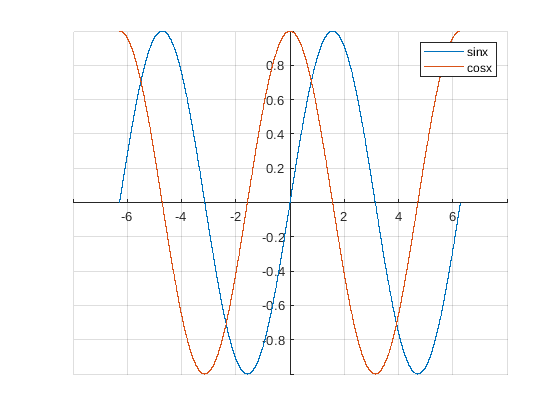
\includegraphics[width=0.5\textwidth]{Analisi1/figures/sincosx.png}
    \caption{Grafico delle funzioni $\sin x$ e $\cos x$.}
    \label{fig:sincosx}
\end{figure}

\begin{definition}[Coseno]
    La funzione
    \begin{equation*}
        \cos x\colon \mathbb R\rightarrow[-1,1]
    \end{equation*}
    rappresenta l'\gls{ascissa} di un punto $P$ (vedere Figura \ref{fig:TrigFunctionDiagram}) descritto dall'angolo $x$ sulla circonferenza goniometrica.
\end{definition}

\begin{proposition}
    Il coseno può essere rappresentato come
    \begin{equation*}
        \cos x=\frac{\overline{\rm OP}}{\overline{\rm OB}}.
    \end{equation*}
\end{proposition}

\begin{definition}[Seno]
    La funzione seno
    \begin{equation*}
        \sin x\colon \mathbb R\rightarrow[-1,1],
    \end{equation*}
    rappresenta l'\gls{ordinata} di un punto $P$ (vedere Figura \ref{fig:TrigFunctionDiagram}) descritto dall'angolo $x$ sulla circonferenza goniometrica.
\end{definition}

\begin{proposition}
    Il seno può essere rappresentato come
    \begin{equation*}
        \sin x=\frac{\overline{\rm PB}}{\overline{\rm OB}}.
    \end{equation*}
\end{proposition}

\begin{property}[Prima relazione fondamentale della goniometria]\label{def:prima_relazione_fondamentale_goniometria}
    Dato che $\sin x$ e $\cos x$ rappresentano, rispettivamente, l'ordinata e l'ascissa del punto della circonferenza goniometrica, vale la \textbf{relazione fondamentale}:
    \begin{equation}
        \cos{x}^2+\sin{x}^2 = 1.
    \end{equation}
\end{property}

\begin{definition}
    La prima relazione fondamentale della trigonometria permette di esprimere le funzioni seno e coseno come segue:
    \begin{equation}\label{eq:prima_relazione_fondamentale_goniometria}
        \begin{matrix}
            \cos^2x=1-\sin^2x,\\
            \sin^2x=1-\cos^2.
        \end{matrix}
    \end{equation}
\end{definition}

\begin{property}
    Le funzioni $\sin x$ e $\cos x$ sono periodiche di periodo $2\pi$. Questo è dovuto alla lunghezza completa della circonferenza, ovvero $2\pi$.
\end{property}

\begin{property}
    La funzione seno è dispari, la funzione coseno è pari.
\end{property}

\begin{definition}[Tangente]
    La funzione tangente è definita come
    \begin{equation*}
        \tan x=\frac{\sin x}{\cos x}\colon \mathbb R\backslash\left\{\frac{\pi}{2}+k\pi,\,k\in\mathbb Z\right\}\rightarrow\mathbb R
    \end{equation*}
    e rappresenta l'ordinata di un punto $T$ (vedere Figura \ref{fig:TrigFunctionDiagram}) descritto dall'angolo $x$ sulla circonferenza goniometrica. 
\end{definition}

I triangoli $OQP$ e $OAT$ sono simili, quindi è possibile definire la seguente proporzione
\begin{equation*}
    \underbrace{\overline{\rm AT}}_{\tan x}\colon\underbrace{\overline{\rm PQ}}_{\sin x}=\underbrace{\overline{\rm OA}}_{1}\colon\underbrace{\overline{\rm OQ}}_{\cos x}.
\end{equation*}

Pertanto, in base alla precedente proporzione è data la Definizione \ref{def:seconda_relazione_fondamentale_goniometria}.

\begin{definition}[Seconda relazione fondamentale della goniometria]\label{def:seconda_relazione_fondamentale_goniometria}
La funzione tangente è definita come
    \begin{equation}\label{eq:seconda_relazione_fondamentale_goniometria}
        \boldsymbol{\tan x=}\frac{\overline{\rm PQ}}{\overline{\rm OQ}}=\boldsymbol{\frac{\sin x}{\cos x}}.
    \end{equation}
\end{definition}

\begin{figure}
    \centering
    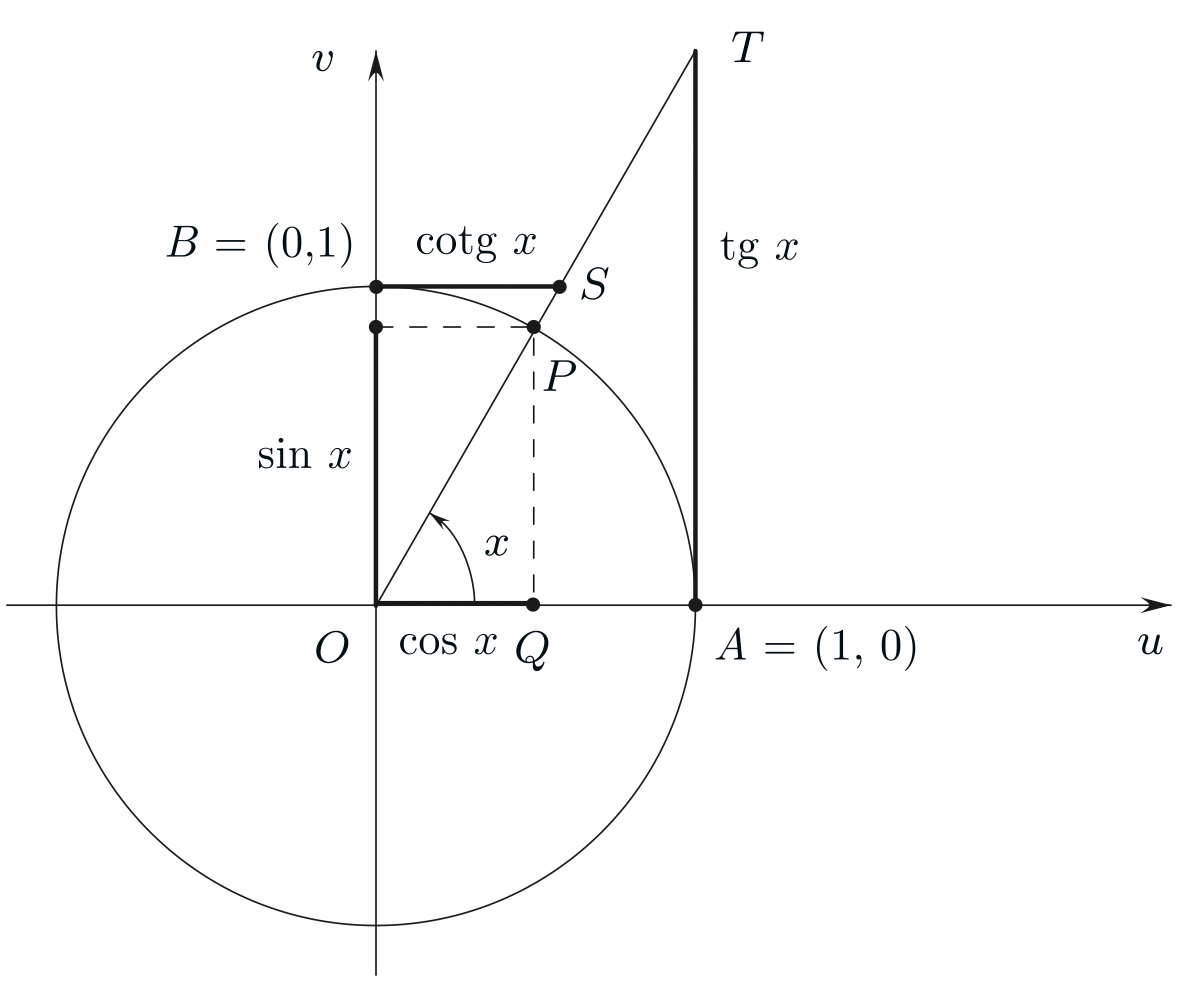
\includegraphics[width=0.5\textwidth]{Analisi1/figures/TrigFunctionDiagram.jpeg}
    \caption{Grafico delle funzioni goniometriche.}
    \label{fig:TrigFunctionDiagram}
\end{figure}

\subsubsection{Funzioni reciproche goniometriche}

\begin{definition}[Cotangente]
    La funzione
    \begin{equation*}
        \cot x = \frac{1}{\tan x}\colon\mathbb R \backslash\{0+k\pi\colon k\in\mathbb N\}\rightarrow\mathbb R
    \end{equation*}
    rappresenta l'ascissa del punto $S$ descritto dall'angolo $x$ sulla circonferenza goniometrica.
\end{definition}

\begin{property}
    La funzione cotangente è una funzione periodica di periodo $\pi$ ed è dispari. Inoltre, la cotangente è il \gls{reciproco} della funzione tangente.
\end{property}


Dato che i triangoli $OQP$ e $OSB$ sono simili, ovvero $\overline{\rm BS}\parallel\overline{\rm OQ}$ e $x'\equiv x$ è possibile definire  la proporzione
\begin{equation*}
    \overline{\rm BS}\colon\overline{\rm OQ}=\underbrace{\overline{\rm OB}}_{1}\colon\overline{\rm PQ}.
\end{equation*}

Pertanto, in base alla precedente proporzione ed alla applicazione del secondo criterio di similitudine dei triangoli \footnote{Gli angoli $x'$ e $x$ sono coincidenti perché alterni interni.} è data la Definizione \ref{def:terza_relazione_fondamentale_goniometria}.

\begin{definition}[Terza relazione fondamentale della goniometria]\label{def:terza_relazione_fondamentale_goniometria}
    La funzione cotangente è definita come
    \begin{equation*}
        \boldsymbol{\cot x=}\frac{\overline{\rm OQ}}{\overline{\rm PQ}}=\frac{1}{\tan x}=\boldsymbol{\frac{\cos x}{\sin x}}.
    \end{equation*}
\end{definition}

Con lo stesso criterio di reciprocità sono definite le seguenti funzioni.

\begin{definition}[Quarta relazione fondamentale della trigonometria]
    La funzione
    \begin{equation*}
        \boldsymbol{\sec x=\frac{1}{\cos x}}\colon\mathbb R\backslash\left\{\frac{\pi}{2}+k\pi\right\}\rightarrow\mathbb R
    \end{equation*}
    rappresenta l'ascissa di un punto $S$ (vedere Figura \ref{fig:circonferenza_goniometrica_secante}) descritto dall'angolo $x$ sulla circonferenza goniometrica.
\end{definition}

\begin{definition}[Cosecante]
    La funzione
    \begin{equation*}
        \csc x=\frac{1}{\sin x}\colon\mathbb R\backslash\left\{\frac{\pi}{2}+k\pi\right\}\rightarrow\mathbb R
    \end{equation*}
    rappresenta l'ordinata di un punto $C$ (vedere Figura \ref{fig:circonferenza_goniometrica_cosecante}) descritto dall'angolo $x$ sulla circonferenza goniometrica.
\end{definition}

\begin{figure}[!hbt]
    \centering
    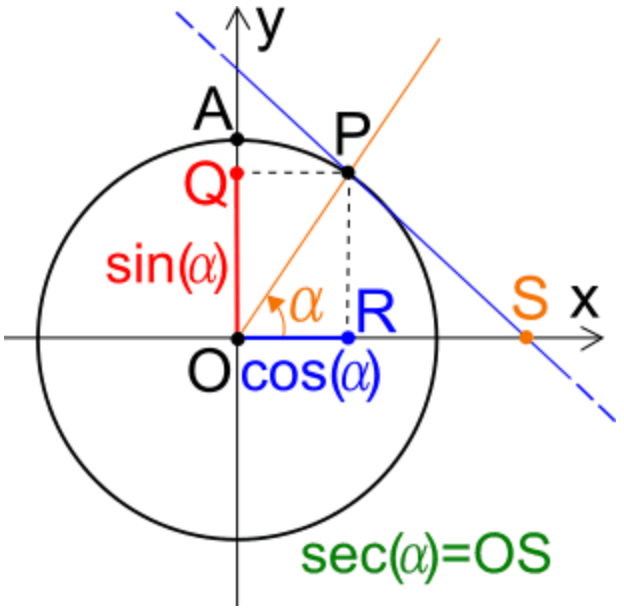
\includegraphics[width=0.5\textwidth]{Analisi1/figures/circonferenza_goniometrica_secante.jpeg}
    \caption{Grafico della funzione $\sec x$.}
    \label{fig:circonferenza_goniometrica_secante}
\end{figure}

\begin{figure}[!hbt]
    \centering
    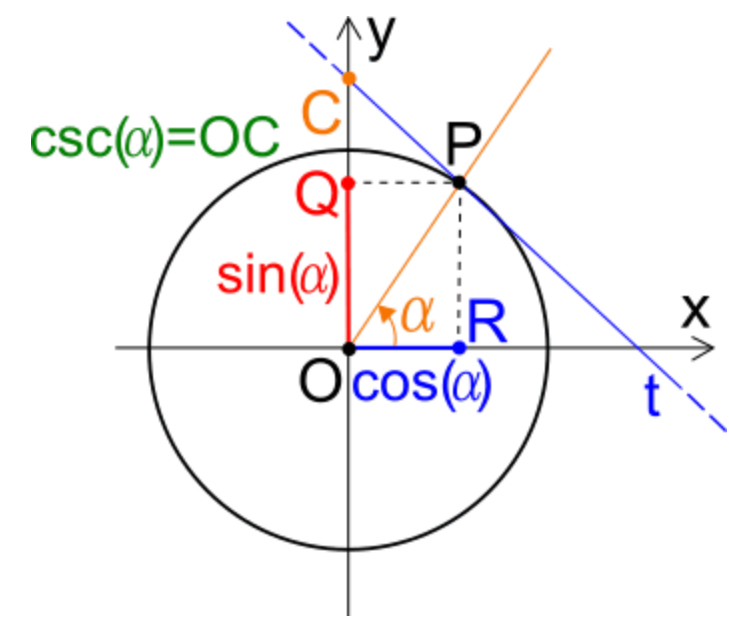
\includegraphics[width=0.5\textwidth]{Analisi1/figures/circonferenza_goniometrica_cosecante.jpeg}
    \caption{Grafico della funzione $\csc x$.}
    \label{fig:circonferenza_goniometrica_cosecante}
\end{figure}

\subsubsection{Formule goniometriche inverse}
Le funzioni gonometriche non sono invertibili, ma selezionando un tratto monotono è possibile definirne le funzioni trigonometriche inverse:

\begin{equation*}
    \arccos x\colon [-1,1]\rightarrow[0,\pi],
\end{equation*}

\begin{equation*}
    \arcsin x\colon [-1,1]\rightarrow\left[-\frac{\pi}{2},\frac{\pi}{2}\right],
\end{equation*}

\begin{equation*}
    \arctan x\colon \mathbb R\rightarrow\left(-\frac{\pi}{2},\frac{\pi}{2}\right).
\end{equation*}

\begin{definition}
    \begin{equation*}
        \begin{matrix}
            \sin(\arctan x) &=& \frac{x}{\sqrt{1+x^2}}\\\\
            \cos(\arccos x) &=& \frac{1}{\sqrt{1+x^2}}.
        \end{matrix}
    \end{equation*}
\end{definition}

\begin{property}
    Le funzioni goniometriche inverse hanno le seguenti proprietà:
    \begin{itemize}
        \item non sono funzioni goniometriche,
        \item hanno come immagine gli angoli in cui valgono le rispettive funzioni.
    \end{itemize}
\end{property}

\begin{figure}
    \centering
    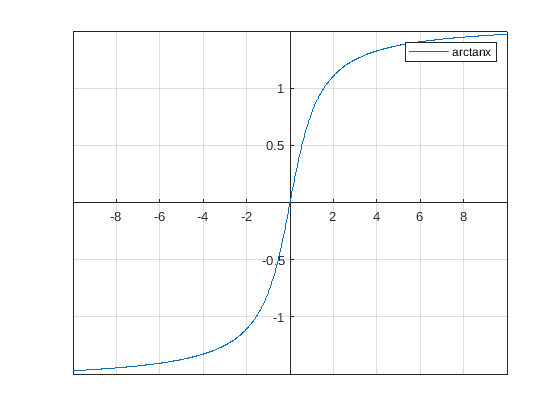
\includegraphics[width=0.5\textwidth]{Analisi1/figures/arctanx.png}
    \caption{Grafico della funzione $\arctan x$.}
    \label{fig:arctanx}
\end{figure}

\begin{figure}
    \centering
    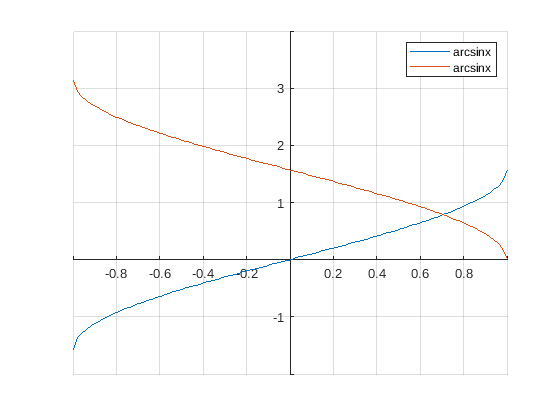
\includegraphics[width=0.5\textwidth]{Analisi1/figures/arcsincosx.png}
    \caption{Grafico delle funzioni $\arcsin x$ e $\arccos x$.}
    \label{fig:arcsincosx}
\end{figure}

\subsubsection{Archi ricorrenti}

\subsubsection{Archi associati}

\textbf{NB:} Saranno utilizzate le Figure \ref{fig:archi_associati1}-\ref{fig:archi_associati} per trattare gli archi associati.

Gli archi associati ad un angolo $\alpha$ è indicato un insieme di formule che permettono di semplificare il calcolo delle funzioni goniometriche.

\begin{definition}
    Dato un angolo $\alpha$, formule sono associate sono definite per i seguenti: $\frac{\pi}{2}-\alpha,\, \frac{pi}{2}+\alpha,\, \pi - \alpha,\, \pi+\alpha,\, \frac{3}{2}\pi-\alpha,\, \frac{3}{2}\pi+\alpha,\, 2\pi - \alpha$.
\end{definition}

Dalla Figura \ref{fig:archi_associati1} è possibile osservare che:
\begin{itemize}
    \item Il punto $P''$ è il simmetrico di $P$ rispetto all'asse $y$.
    \item Il punto $P^{iv}$ è simmetrico di $P$ rispetto all'asse $x$.
    \item Il punto $P'''$ è il simmetrico di $P$ rispetto all'origine.
\end{itemize}

\begin{figure}
    \centering
    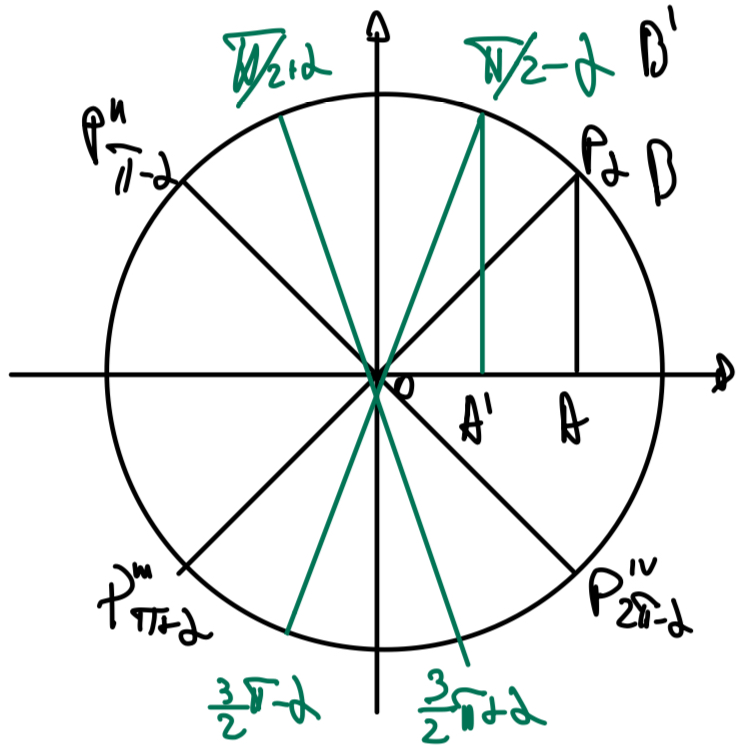
\includegraphics[width=0.5\textwidth]{Analisi1/figures/archi_associati1.jpeg}
    \caption{Archi associati}
    \label{fig:archi_associati1}
\end{figure}

\begin{figure}
    \centering
    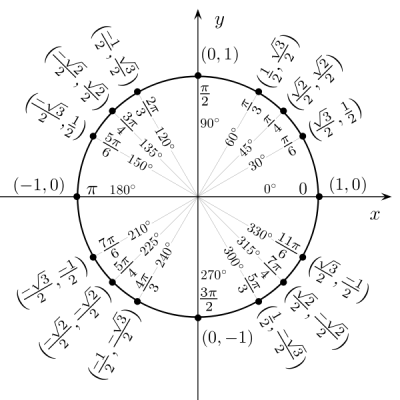
\includegraphics[width=0.5\textwidth]{Analisi1/figures/archi_associati.png}
    \caption{Archi associati}
    \label{fig:archi_associati}
\end{figure}

\paragraph{Angoli opposti e supplementari}
\begin{definition}[Angolo opposto]
    L'angolo opposto di $\alpha$ è $-\alpha$.
\end{definition}

\begin{definition}[Angolo esplementare]
    L'angolo esplementare di $\alpha$ è un angolo che sommato ad $\alpha$ è uguale a $2\pi$.
\end{definition}

Angolo esplementare ed angolo opposto coincidono nel contesto della circonferenza goniometrica in quanto $-\alpha=(0-\alpha)=2\pi-\alpha$.

\begin{definition}[Archi associati per $\alpha$]
    \begin{equation*}
        \begin{matrix}
            \sin(-\alpha)&=&-\sin\alpha,\\
            \cos(-\alpha)&=&\cos(\alpha),\\
            \tan(-\alpha)&=&-\tan(\alpha),\\
            \cot(-\alpha)&=&-\cot(\alpha).
        \end{matrix}
    \end{equation*}
\end{definition}

\paragraph{Archi supplementari}
\begin{definition}[Archi associati per $\pi-\alpha$]
    \begin{equation*}
        \begin{matrix}
            \sin(\pi-\alpha)&=&\sin(\alpha),\\
            \cos(\pi-\alpha)&=&-\cos(\alpha),\\
            \tan(\pi-\alpha)&=&-\tan(\alpha),\\
            \cot(\pi-\alpha)&=&-\cot(\alpha).
        \end{matrix}
    \end{equation*}
\end{definition}

\begin{definition}[Archi associati $\pi+\alpha$]
    \begin{equation*}
        \begin{matrix}
            \sin(\pi+\alpha)&=&-\sin(\alpha),\\
            \cos(\pi+\alpha)&=&-\cos(\alpha),\\
            \tan(\pi+\alpha)&=&\tan(\alpha),\\
            \cot(\pi+\alpha)&=&\cot(\alpha).
        \end{matrix}
    \end{equation*}
\end{definition}

\paragraph{Angoli complementari}

\begin{definition}[Archi associati $\frac{\pi}{2}-\alpha$]
    \begin{equation*}
        \begin{matrix}
            \sin\left(\frac{\pi}{2}-\alpha\right)&& &=& &&\cos(\alpha),\\
            \cos\left(\frac{\pi}{2}-\alpha\right)&& &=& &&\sin(\alpha),\\
            \tan\left(\frac{\pi}{2}-\alpha\right)&=&\frac{\sin\left(\pi-\alpha\right)}{\cos\left(\pi-\alpha\right)}&=&\frac{\cos(\alpha)}{\sin(\alpha)}&=&\cot(\alpha)\\
            \cot\left(\frac{\pi}{2}-\alpha\right)&=&\frac{\cos(\pi-\alpha)}{\sin(\pi-\alpha)}&&&=&\tan\alpha.
        \end{matrix}
    \end{equation*}
\end{definition}

Le precedenti formule sono dovute al fatto che $B'$ e $B$ sono congruenti ed i triangoli $OAB$ e $OA'B'$ siano simili (sono lo stesso traslato in quanto $\overline{\rm A'B'}=\overline{\rm OA}$ e $\overline{\rm OA}=\overline{\rm AB}$).

Traslando il triangolo $OA'B'$ nel secondo quadrante è ottenuto quanto segue.

\begin{definition}[Archi associati $\frac{\pi}{2}+\alpha$]
    \begin{equation*}
        \begin{matrix}
            \sin\left(\frac{\pi}{2}+\alpha\right)&& &=& &&\cos(\alpha),\\
            \cos\left(\frac{\pi}{2}+\alpha\right)&& &=& &&-\sin(\alpha),\\
            \tan\left(\frac{\pi}{2}+\alpha\right)&=&\frac{\sin\left(\pi+\alpha\right)}{\cos\left(\pi+\alpha\right)}&=&\frac{\cos(\alpha)}{-\sin(\alpha)}&=&-\cot(\alpha),\\
            \cot\left(\frac{\pi}{2}+\alpha\right)&=&\frac{\cos(\pi+\alpha)}{\sin(\pi+\alpha)}&&&=&-\tan\alpha.
        \end{matrix}
    \end{equation*}
\end{definition}

Traslando i quadranti sono ottenute le seguenti definizione.

\begin{definition}[Archi associati per $\frac{3\pi}{2}-\alpha$]
    \begin{equation*}
        \begin{matrix}
            \sin\left(\frac{3\pi}{2}-\alpha\right)&\overset{\frac{3\pi}{2}=-\frac{\pi}{2}}{=}& \sin\left(-\frac{\pi}{2}-\alpha\right)&=&\sin\left[-\left(\frac{\pi}{2}+\alpha\right)\right]\overset{\footnotemark}{=}-\cos\alpha,\\
            \cos\left(\frac{3\pi}{2}-\alpha\right)&=&&=&-\sin\alpha,\\
            \tan\left(\frac{3\pi}{2}-\alpha\right)&=& &=&\cot\alpha,\\
            \cot\left(\frac{3\pi}{2}-\alpha\right)&=&&=&\tan\alpha.
        \end{matrix}
    \end{equation*}
\end{definition}
\footnotetext{$\sin(-\alpha)=-\sin\alpha$.}

\begin{definition}[Archi associati per $\frac{3\pi}{2}+\alpha$]
    \begin{equation*}
        \begin{matrix}
            \sin\left(\frac{3\pi}{2}+\alpha\right)&\overset{\frac{3\pi}{2}=-\frac{\pi}{2}}{=}& \sin\left(-\frac{\pi}{2}+\alpha\right)&=&\sin\left[-\left(\frac{\pi}{2}-\alpha\right)\right]&\overset{\footnotemark}{=}&-\cos\alpha,\\
            \cos\left(\frac{3\pi}{2}+\alpha\right)&=&&=&\sin\alpha,\\
            \tan\left(\frac{3\pi}{2}+\alpha\right)&=& &=&-\cot\alpha,\\
            \cot\left(\frac{3\pi}{2}+\alpha\right)&=&&=&-\tan\alpha.
        \end{matrix}
    \end{equation*}
\end{definition}

\subsubsection{Formule parametriche del seno e coseno}
Le formule parametriche permettono di esprimere il seno ed il cose in funzione di $\tan\left(\frac{\alpha}{2}\right)$ e sono utili anche per il calcolo integrale.
\begin{definition}[Formula parametrica di $\sin x$]
    \begin{equation}\label{eq:formula_parametrica_seno}
        \begin{matrix}
            \boldsymbol{\sin\alpha}&\boldsymbol =& \sin\left[2\left(\frac{\alpha}{2}\right)\right] &\overset{\ref{eq:formula_duplicazione_seno}}{=}& 2\sin\frac{\alpha}{2}\cos\frac{\alpha}{2}&\equiv&\frac{2\sin\frac{\alpha}{2}\cos\frac{\alpha}{2}}{1}&\overset{(\ref{eq:prima_relazione_fondamentale_goniometria})}{=}&\frac{2\sin\frac{\alpha}{2}\cos\frac{\alpha}{2}}{\underbrace{\sin^2\frac{\alpha}{2}+\cos^2\frac{\alpha}{2}}_{\footnotemark}} \\
            && &\overset{\footnotemark}{=}& \frac{\frac{2\sin\frac{\alpha}{2}\cancel{\cos\frac{\alpha}{2}}}{\cos^{\cancel{2}}\frac{\alpha}{2}}}{\underbrace{\frac{\sin^2\frac{\alpha}{2}+\cos^2\frac{\alpha}{2}}{\cos^2\frac{\alpha}{2}}}_{\footnotemark}}&=& \frac{\frac{2\sin\frac{\alpha}{2}}{\cos\frac{\alpha}{2}}}{\frac{\sin^2\frac{\alpha}{2}}{\cos^2\frac{\alpha}{2}}+\frac{\cancel{\cos^2\frac{\alpha}{2}}}{\cancel{\cos^2\frac{\alpha}{2}}}}&=& \boldsymbol{\frac{2\tan\frac{\alpha}{2}}{\tan^2\frac{\alpha}{2}+1}}
        \end{matrix}
    \end{equation}
\end{definition}

\begin{definition}[Formula parametrica di $\cos x$]
    \begin{equation}\label{eq:formula_parametrica_coseno}
        \begin{matrix}
            \boldsymbol{\cos\alpha} &=& \cos\left[2\left(\frac{\alpha}{2}\right)\right] &=& \cos^2\frac{\alpha}{2}-\sin^2\frac{\alpha}{2} &\equiv& \frac{\cos^2\frac{\alpha}{2}-\sin^2\frac{\alpha}{2}}{1} \\\\
            && &=& \frac{\cos^2\frac{\alpha}{2}-\sin^2\frac{\alpha}{2}}{\sin^2\frac{\alpha}{2}+\cos^2\frac{\alpha}{2}} &=& \frac{\frac{\cos^2\frac{\alpha}{2}-\sin^2\frac{\alpha}{2}}{\cos^2\frac{\alpha}{2}}}{\frac{\sin^2\frac{\alpha}{2}+\cos^2\frac{\alpha}{2}}{\cos^2\frac{\alpha}{2}}}&=&\boldsymbol{\frac{1-\tan^2\frac{\alpha}{2}}{1+\tan^2\frac{\alpha}{2}}}
        \end{matrix}
    \end{equation}
\end{definition}

\addtocounter{footnote}{-2}
\footnotetext{L'angolo della prima relazione fondamentale della goniometria (\ref{eq:prima_relazione_fondamentale_goniometria}) può essere qualsiasi, quindi è scelto $\frac{\alpha}{2}$.}

\stepcounter{footnote}
\footnotetext{Moltiplicazione e divisione per $\cos^2\frac{\alpha}{2}$ con la condizione che $\cos^2\frac{\alpha}{2}\neq 0$. La condizione si verifica se $\alpha\neq\frac{\pi}{2}+k\pi$, quindi se $\alpha\neq\pi$.}

\stepcounter{footnote}
\footnotetext{Proprietà distributiva della divisione.}

Le formule (\ref{eq:formula_parametrica_seno}) e (\ref{eq:formula_parametrica_coseno}) possono essere considerate, utilizzando l'uguaglianza
\begin{equation*}
    \tan\frac{\alpha}{2}=t,
\end{equation*}

come segue
\begin{equation*}
    \begin{matrix}
        \sin\alpha &=& \frac{2t}{t^2+1},\\
        \\
        \cos\alpha &=& \frac{1-t^2}{1+t^2}.
    \end{matrix}
\end{equation*}

\subsubsection{Formule di addizione e sottrazione}
\begin{definition}[Formula addizione e sottrazione $\sin x$]
    \begin{equation}\label{eq:addizione_sottrazione_seno}
        \sin(\alpha\pm\beta)=\sin\alpha\cos\beta\pm\sin\beta\cos\alpha.
    \end{equation}
\end{definition}

\begin{definition}[Formula addizione e sottrazione $\cos x$]
    \begin{equation}\label{eq:addizione_sottrazione_coseno}
        \cos(\alpha\pm\beta)=\cos\alpha\cos\beta\mp\sin\alpha\sin\beta.
    \end{equation}
\end{definition}

\begin{definition}[Formula addizione e sottrazione $\tan x$]
    \begin{equation}\label{eq:addizione_sottrazione_tangente}
        \tan(\alpha\pm\beta)=\frac{\tan\alpha+\tan\beta}{1\mp\tan\alpha\tan\beta}.
    \end{equation}
\end{definition}

\paragraph{Intermezzo passaggi $\boldsymbol{\tan(\alpha\pm\beta)=\frac{\tan\alpha+\tan\beta}{1\mp\tan\alpha\tan\beta}}$:}
\begin{equation*}
    \begin{matrix}
        \boldsymbol{\tan(\alpha+\beta)}&\overset{(\ref{eq:seconda_relazione_fondamentale_goniometria})}{=}&\frac{\sin(\alpha+\beta)}{\underbrace{\cos(\alpha+\beta)}_{\footnotemark}}&\overset{(\ref{eq:addizione_sottrazione_seno})-(\ref{eq:addizione_sottrazione_coseno})}{=}&\frac{\sin\alpha\cos\beta+\sin\beta\cos\alpha}{\cos\alpha\cos\beta-\sin\alpha\sin\beta}\\
        &\overset{\footnotemark}{=}&\frac{\frac{\sin\alpha\cos\beta}{\cos\alpha\cos\beta}+\frac{\cos\alpha\cos\beta}{\cos\alpha\cos\beta}}{\frac{\cos\alpha\cos\beta}{\cos\alpha\cos\beta}-\frac{\sin\alpha\sin\beta}{\cos\alpha\cos\beta}}&=&\frac{\frac{\sin\alpha}{\cos\alpha}+\frac{\sin\beta}{\cos\beta}}{1-\frac{\sin\alpha}{\cos\beta}\frac{\sin\beta}{\cos\beta}}&=&\boldsymbol{\frac{\tan\alpha+\tan\beta}{1-\tan\alpha\tan\beta}},
    \end{matrix}
\end{equation*}

\addtocounter{footnote}{-1}
\footnotetext{La condizione è che $\cos(\alpha-\beta)$, ovvero $\alpha+\beta\neq\frac{\pi}{2}+k\pi$.}

\stepcounter{footnote}
\footnotetext{Divisione per $\cos\alpha\cos\beta$, supponendo $\alpha\neq\frac{\pi}{2}+k'\pi$ e $\beta\neq\frac{\pi}{2}+k''\pi$.}

\begin{equation*}
    \tan(\alpha-\beta)=\tan(\alpha+(-\beta))=\frac{\tan\alpha+\tan(-\beta)}{1-\tan\alpha\tan\beta}=\frac{\tan\alpha+\tan\beta}{1+\tan\alpha\tan\beta}.
\end{equation*}

\begin{example}
    $\sin(15^\circ)=\sin(\frac{\pi}{4}-\frac{\pi}{6})=\sin\frac{\pi}{4}\cos\frac{\pi}{6}-\sin\frac{\pi}{6}\cos\frac{\pi}{4}=\frac{\sqrt{6}-\sqrt{2}}{4}=\frac{\sqrt{2}}{2}\cdot-\frac{1}{2}\cdot\frac{\sqrt{2}}{2}$.
\end{example}

\begin{remark}
    Le formule degli archi associati sono casi particolari delle formule precedenti.
\end{remark}

\begin{example}
    $\sin(\pi-\alpha)=\underbrace{\sin\pi}_{0}\cos\alpha-\sin\alpha\underbrace{\cos\pi}_{-1}=\sin\alpha$.
\end{example}


\subsubsection{Formule di duplicazione}
Le formule i duplicazione sono casi particolari delle formule di addizione e sottrazione.

\begin{definition}[Formula duplicazione $\sin x$]
    \begin{equation}\label{eq:formula_duplicazione_seno}
        \sin(2\alpha)=\sin(\alpha+\alpha)=2\sin\alpha\cos\alpha.
    \end{equation}
\end{definition}

\begin{definition}[Formula duplicazione $\cos x$]\label{def:formula_duplicazione_coseno}
    \begin{equation}\label{eq:formula_duplciazione_coseno}
        \cos(2\alpha)=\cos(\alpha+\alpha)=\cos^2\alpha-\sin^2\alpha\overset{(\ref{eq:prima_relazione_fondamentale_goniometria})}{=}
        \begin{cases}
            2\cos^2\alpha-1,\\
            1-2\sin^2\alpha.
        \end{cases}
    \end{equation}
\end{definition}

\begin{definition}[Formula duplicazione $\tan x$]
    \begin{equation*}
        \tan(2\alpha)=\tan(\alpha+\alpha)=\frac{\tan\alpha+\tan\alpha}{1-\tan\alpha\tan\alpha}=\frac{2\tan\alpha}{1-\tan\alpha}.
    \end{equation*}
\end{definition}

E' possibile utilizzare la formula di duplicazione del coseno per esprimere in modo diverso $\sin^2\alpha$ e $\cos^2\alpha$.
\begin{remark}
    Sia, dalla Definizione \ref{def:formula_duplicazione_coseno}, $\cos(2\alpha)=1-\sin^2\alpha$ allora
    \begin{equation}
        \begin{matrix}
            \sin^2\alpha=\frac{1-\cos(2\alpha)}{2}\rightarrow\sin\alpha=\pm\sqrt{\frac{1-\cos(2\alpha)}{2}}\\
            \cos^2\alpha=\frac{1+\cos(2\alpha)}{2}\rightarrow\cos\alpha=\pm\sqrt{\frac{1-\cos(2\alpha)}{2}}
        \end{matrix}
    \end{equation}
\end{remark}

\subsubsection{Formule di prostaferesi}
Le formule di prostaferesi sono formule goniometriche che consentono di trasformare la somma e la differenza di due seni o di due coseni in un prodotto tra seno e coseno.
\begin{definition}[Per il seno]
    \begin{equation*}
        \begin{matrix}
            \sin(\alpha)+\sin(\beta) &=& 2 \sin\left(\frac{\alpha+\beta}{2}\right)\cdot\cos \left(\frac{\alpha-\beta}{2}\right)\\
            \sin(\alpha)-\sin(\beta) &=& 2 \cos\left(\frac{\alpha+\beta}{2}\right)\cdot\sin \left(\frac{\alpha-\beta}{2}\right)
        \end{matrix}
    \end{equation*}
\end{definition}

\begin{definition}[Per il coseno]
    \begin{equation*}
        \begin{matrix}
            \cos\alpha+\cos\beta &=& 2\cos\left(\frac{\alpha+\beta}{2}\right)\cos\left(\frac{\alpha -\beta}{2}\right)\\
            \cos\alpha-\cos\beta &=& -2\sin\left(\frac{\alpha+\beta}{2}\right)\sin\left(\frac{\alpha -\beta}{2}\right)
        \end{matrix}
    \end{equation*}
\end{definition}

\subsubsection{Formule di bisezione}
Le formule di bisezione sono ricavate dalla formula di duplicazione del seno sostituendo $\alpha$ con $\frac{\alpha}{2}$.

\begin{definition}
    \begin{equation*}
        \begin{matrix}
            \sin\left(\frac{\alpha}{2}\right)&=&\pm\sqrt{\frac{1-\cos\alpha}{2}},\\
            \cos\left(\frac{\alpha}{2}\right)&=&\pm\sqrt{\frac{1+\cos\alpha}{2}},
        \end{matrix}
    \end{equation*}
    \begin{equation*}
        \tan\left(\frac{\alpha}{2}\right)=\frac{\sin\frac{\alpha}{2}}{\frac{\cos\alpha}{2}}=\frac{\pm\sqrt{\frac{\-\cos\alpha}{2}}}{\pm\sqrt{\frac{1+\cos\alpha}{2}}}=\pm\sqrt{\frac{1-\cos\alpha}{1+\cos\alpha}}.
    \end{equation*}
\end{definition}

\subsubsection{Formule di Werner}
Le formule di Werner sono ricavate sommando membro a membro le formule di addizione.

\begin{definition}
    \begin{equation*}
        \begin{matrix}
            \sin\alpha\sin\beta &=& \frac{1}{2}[\cos(\alpha-\beta)-\cos(\alpha+\beta)],\\\\
            \cos\alpha\cos\beta &=& \frac{1}{2}[\cos(\alpha+\beta)+\cos(\alpha-\beta)],\\\\
            \sin\alpha\cos\beta &=& \frac{1}{2}[\sin(\alpha+\beta)+\sin(\alpha-\beta)].
        \end{matrix}
    \end{equation*}
\end{definition}